\chapter{Transformer Architecture and LLMs}\label{ch_transformers}
\chapterauthor{Pierre Beckmann, Tim Meyer, Jeff Yoshimi}{.2, .2, .6}

% TODO: Watch new 3b1b videos and add note.  (Maybe say we will do more to cohere in the next revision for better interpretation). For example, think of each head as asking a question. Gets us intuition about self attention. Also each attention head looks at something different. Queries are like questions, keys are like replies.
%TODO: Encoders, decoders, masking, other cases. For example, we can feed a transformer network the first halves of hundreds of movie scripts and train it to produce the second halves of those scripts, or we can train it to predict what the first summary paragraph of a Wikipedia article is based on the main body of the article. Cohere this with the point about BERT being bidirectional at the end of the section. Search "unidirectional"

As discussed in the history section \extref{age_generative_ai}, we have entered a new stage in the history of neural networks, what we are calling the ``age of generative AI'', which is familiar via transformer-based LLM's like ChatGPT.  GPT as a generic term means “Generative Pre-trained Transformer” (though it is often also used to refer specifically to open AI’s models). Though the transformer architecture can be used in many ways, it became prominent through its use to support large language models (LLMs), which are language models that generate human readable text.\footnote{As noted in section \extref{age_generative_ai}, the two terms are often conflated. To be clear, the transformer is the neural network architecture, while an LLMs is just any model of language generation that is based on a large dataset.  But they are distinct concepts. An LLM can be built out of something besides a transformer, and transformers can be used on things besides language. For example, state of the art image classification models are now transformer-based, and OpenAI has released an impressive video generation model – Sora, which also runs on a transformer architecture.} We will sometimes use the term ``GPT'' as a covering term for transformer-based LLMs because the majority of the current popular LLMs are GPTs.  We will also sometimes refer simply to ``LLMs'' by which we mean transformer-based LLMs. But our preferred term is ``transformer based LLM.''\footnote{There are many different models in this class. As of this writing (June 2024), this includes the open Ai GPT series: GPT, GPT2, GPT3, GPT4, and GPT 4o.  It also  includes BERT (Google’s first LLM, which is now out-dated). Gemini  (Bard), several Claude models (Anthropic;  semi open-source), Llama, LLama2 and LLama3 (Meta), and Alpaca (Stanford; open source). Most of these models can only be accessed online but some can be downloaded and run locally, further fine-tuned, etc.}

Earlier efforts at text generation and natural language processing used supervised recurrent networks (chapter \extref{ch_supervised_recurrent}), which are in various ways limited. The transformer architecture is basically a very complex feed-forward network. By using feed-forward networks to train language models, all the accumulated insights of decades of research could be leveraged in this domain, where contextual representations are so important. These models generate text responses to text inputs by repeatedly predicting the next word in a sequence. They are trained on large datasets of everyday text, like text from the internet, which is easily available. They often use a transformer architecture, which is a many-layered feed-forward network with special mechanisms for learning relationships between inputs. This architecture draws on the lesson of the deep learning revolution (section \extref{deep_revolution}), using many layered deep networks (chapter \extref{ch_cnn}) that develop complex representation (they make good use of both ``representational width" and ``representational depth''). They can be trained on large datasets using highly optimized parallel hardware.  And like all the other networks discussed in this book, they are not just useful as engineered tools, but are highly relevant both to neuroscience and cognitive science, and seem to develop meaningful internal representations. 

We start with preliminary discussion of how transformer-based LLMs are trained using highly available text data, and how a special recursive trick can be used to make a feed-forward network that only predicts next words still produce meaningful conversational outputs. We then discuss how the transformer architecture itself works.  Finally we consider how LLMs are utilized and evaluated and the relevance of these models to cognitive science, neuroscience and other areas.

Changes in this area are rapid, and the relevance of these areas to cognitive science is only now being studied, so updates to this chapter are expected (in fact a fairly detailed development of the core graphics is currently underway).

\section{Learning to speak Internetese}

In section \extref{languageModelsRecurrent} we saw how language models trained on example text would learn to speak in a certain way that reflects the statistical properties of the training data. A network trained on Shakespeare would start to speak fake Shakespeare, fake math was generated, etc. 
Large language models using transformers do the same thing, they just do it much better. They use larger datasets (hence ``large'' being added in front of ``language model''), and they use a feed-forward transformer architecture that, as of this writing, outperforms recurrent architectures. 

% TODO Check
The training set for GPT-3 is not all of Shakespeare, or a bunch of math papers, but a much larger dataset that encompasses both of those and much, much more (see figure \ref{gptDatasets}).  In particular, it includes all of Wikipedia, a few compilations of books, and a web-scraped archive of a large subset of the \emph{entire internet}, called common crawl (\url{https://en.wikipedia.org/wiki/Common_Crawl}.) If you've ever written anything online, there is a decent chance it is part of the training data that was used! It is an absolutely massive dataset. Using next-word prediction on a whole dataset can be converted into a labeled dataset, just using this freely available text.  Also the network used to process it is massive (see figure \ref{gptParams}). 

Since all of Shakespeare is on the internet, and discussions of every topic of human endeavor from physics to history, and plenty of gossip and randomness about popular culture and everything else, it can talk about all of these things.  It can statistically generalize from its training data, which in this case is primarily a large part of the internet. Thus, in a sense, it learns to speak ``internetese''.  (Also note that common crawl and GPT-4 are regularly updated, so it stays up to date within a year-or-two). 
% Reference above

% TODO: This and the one below
\begin{figure}[h]
\centering
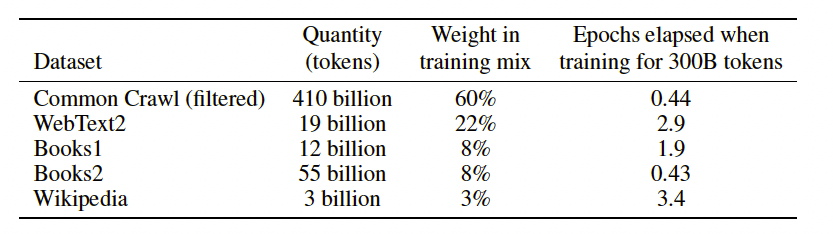
\includegraphics[scale=.4]{./images/gptDatasets}
\caption[GPT Technical report. Todo]{The datasets used to train GPT-3. Mostly internet, but lots of books and all of Wikipedia too. }
\label{gptDatasets}
\end{figure}

% Turing test more citations
The results are impressive. The texts it produces are no longer obviously fake in the way the examples from section \extref{languageModelsRecurrent} were. In fact, in some cases it arguably passes the Turing Test, a long-standing test for artificial general intelligence, answering questions and producing convincing  text in response to prompts.\footnote{\url{https://plato.stanford.edu/entries/turing-test/}. Whether GPT really passes the test is a matter of ongoing controversy.} For example, when asked to write an article with the title ``United Methodists Agree to Historic Split: Those who oppose gay marriage will form their own denomination'', it produced the following:
\begin{quote}
After two days of intense debate, the United Methodist Church has agreed to a historic split - one that is expected to end in the creation of a new denomination, one that will be ``theologically and socially conservative,'' according to The Washington Post. The majority of delegates attending the church's annual General Conference in May voted to strengthen a ban on the ordination of LGBTQ clergy and to write new rules that will "discipline" clergy who officiate at same-sex weddings. But those who opposed these measures have a new plan: They say they will form a separate denomination by 2020, calling their church the Christian Methodist denomination...
\end{quote}
Most people can't tell that this was written by a computer.  This kind of text generation was big news back in 2020, but of course, it's run-of-the-mill now that we are all familiar with GPT.

\section{Training Using Next-Word Prediction}

So how do the mechanics of all this work in practice? Recall from chapter \extref{ch_data_science} that a training dataset consists of inputs and targets, and is also called a labeled dataset. This kind of labeled data can be hard to get, as we saw.  We might have lots of pictures of people but not know the names or identities of the people in the pictures, or lots of pictures of cats and dogs but not whether a given picture is a cat or dog.  This method (sometimes known as auto-regression) provides a way to take \emph{any piece of text} and convert it into a training data set. The trick is to take a set of tokens in a text as input, and then to use the next token as the target, or label.  Any text will do! For example, consider this block of text adapted from the Wikipedia page for UC Merced:

\begin{quote}
The University of California, Merced is a public land-grant research university in Merced, California. It is one of the ten campuses in the University of California (UC) system. Established in 2005, Merced is the newest campus within the UC system.
\end{quote}

From this can create a bunch of training examples, a bunch of input / target pairs. We might use ``The University of" as an input, and then ``California'' as a target.  We simply associate each token in the input with a vector using a word embedding, and the target with an embedding, and we can build a table of input-target vector pairs, which we can use to train a feed-forward neural network.  For a sense of the idea, see figure \ref{nextWordPrediction}.\footnote{Note that normally a word like ``University'' would be split into multiple tokens, but we are keeping things simple here. Some information tokenizers is in chapter \extref{ch_word_embeddings}.}  Note that we are showing the targets as token embeddings that match the inputs, though in practice transformers treat the outputs differently than the inputs, using softmax and one-hot encodings, as we'll see.

\begin{figure}[h]
\centering
\includegraphics[scale=.45]{./images/nextWordPrediction.png}
\caption[Jeff Yoshimi]{A schematic view of how text sequences can be converted into training datasets for large language models. A set of tokens is converted into vectors using a token embedding, and we can treat each concatenated partial sequence of token embeddings as an input and the next token as a target for supervised learning algorithm. }
\label{nextWordPrediction}
\end{figure}
  
\section{How Text is Generated from a Feed-Forward Network}

We've seen the basics of how training works. But now how do we use these models to produce text output? One potentially confusing thing about figure \ref{nextWordPrediction} is that we go from a large input covering a whole set of tokens to a single word output. In fact, in hearing about generative AI as "next word prediction" machines, you may have sometimes wondered how such complicated things can happen when all they model does is predict next words. The answer is by using a key trick at the basis of the whole enterprise, what we can call the ``recursion trick''.  This trick allows us to take a feed-forward network (albeit a very complicated one) that only predicts next words, as above, but use it in a way that produces  streams of text output.

Here is how it works. We feed a network a set of inputs corresponding to a set of tokens (word embeddings of tokens), and it produces an output corresponding to a single token. That output is then appended to the previous input, and this longer input is now fed back to the network. This process is repeated to produce a stream of text outputs. 

How can we put larger and larger inputs into the network? The answer is that we simply specify a fixed length \glossary{context window}, that starts off all zeros, and gets progressively filled in. When you run out of slots you simply remove things from the start of the context window and add to the end (from a computer science standpoint, this is a queue). This is intuitive in figures \ref{nextWordPrediction} and \ref{gptRecursedInputs}.\footnote{Notice that this is a kind of recurrence, and arguably this makes LLMs used in this way a kind of recurrent network. Outputs are fed back in as part of inputs. However, the outputs are text which then must be converted back to text inputs which are then vector encoded.  In fact, recurrent networks were originally used for text processing, as we saw in chapter \extref{ch_supervised_recurrent},but it turns out fancy feedforward networks used in this way outerperform them.  (In those cases a vector representation of each token in the sequence would be presented separately: ``hello'', ``how'', ``are'', ``you'', and ``?''.).}

 GPT-3 has a context window of about 2000 tokens or about 6 pages of text, and early versions of GPT-4 had context windows of 32,000 tokens or about 72 pages of text.  

This technique can be used to generate unending sequences of text from any prompt. The prompt is our input, and then answers are generated using the recursion trick. Text will continue to be generated until a special end of sequence token is reached. It was an important step forward with GPT-3 when the ability to produce end of sequence tokens in a way that mimic human conversation or ``chat'' was produced. This was done using special training techniques that go beyond the topics of this chapter.\footnote{RLHF, reinforcement learning with human feedback, which uses reinforcement learning and policy gradient descent, with a human in the loop. This was introduced with GPT-3.} 

In a dialog, the prompts from the person and the responses from the LLM are both included until the context window is filled. Thus, if the context window is large enough, whole series of back and forth conversations can be processed.  All the prompts and responses up until the current point are part of the input, and then the LLM uses the recursion trick to generate new responses that are sensitive to everything that's been discussed thus far.
% Need pictures for this

Suppose we want to ask a network ``hello how are you?'' The input to the network is the whole sentence $\{$``hello'', ``how'', ``are'', ``you'', ``?''$\}$. Let's  not worry about the vector embeddings, and just see the general idea, as shown in figure \ref{gptRecursedInputs}. Notice that the initial prompt is the initial input, but then the prompt \emph{and} the first word of the response are used as the next input, and this process can be repeated until a response is written out.
  
\begin{figure}[h]
\centering
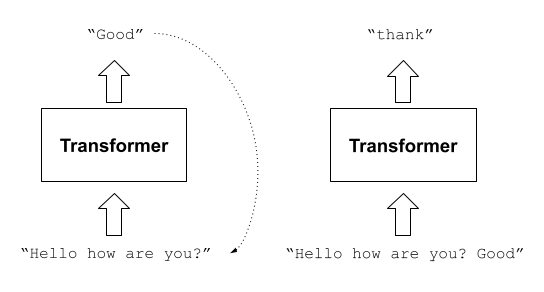
\includegraphics[scale=.7]{./images/gptRecursedInputs.png}
\caption[Jeff Yoshimi]{A schematic view of how ``conversations'' are generated from a feed-forward network in systems like GPT. The output from one moment is added to the end of the input, and the new input is then fed in. The process is repeated to generate a full response.}
\label{gptRecursedInputs}
\end{figure}

\section{The Transformer Architecture}\label{transformers}

So, how does the fancy feed-forward network at the heart of these models work? Their power rests on a few novel architectural innovations, which combine \glossary{representational width} and \glossary{representational depth} with a special form of context awareness. All the things we've seen about other neural networks apply here. It is a kind of deep feed-forward network, which uses a huge amount of training data. But the key innovation is that within each ``layer'' it can develop many forms of context representation, which relate all the tokens in a context window to each other.

\subsection{Blocks}

The transformer architecture \cite{vaswani2017attention} contains layers or ``blocks'' which are specialized to process the large context windows that are fed to the network as input. With training they learn to find long-range dependencies between different parts of a context window. Recall that the context window  includes an original prompt, its own response to that prompt, etc.; it includes the \emph{entire exchange} you've had with GPT up to the current point, so long as it fits in the context window. Each block combines  a ``self-attention'' layer with a traditional linear layer and several other mechanisms (see figure \ref{transformerBlockSimple}). The self-attention layer is where the magic happens. One part of this layer compares each token in the context window to every other token in the window. In our simple example, ``hello'' is compared to ``hello'', ``how'', ``are'', and ``you'', and this comparison is used to create a representation of the sentence that reflects dependencies between the words. All words are compared to each other in the context window, so that no matter how far apart they are, they can still influence each other. The self-attention mechanism learns what relations between words in a context window are important; in a sense it learns what to focus on (hence ``self attention''). This ability to find meaningful relationships within an input sequence is part of why transformers are relevant to cognitive science, as we will see.

\begin{figure}[h]
\centering
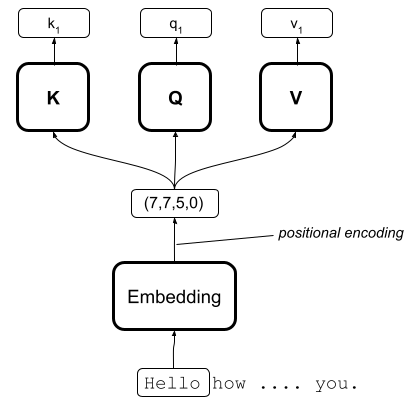
\includegraphics[scale=.4]{./images/transformerBlockBasic.png}
\caption[Jeff Yoshimi with consultation from Tim Meyer.]{Part of one head of a transformer block. Each token is converted into a vector using a word embedding. This vector is then multiplied by three matrices  $\textbf{V}$, $\textbf{Q}$, and $\textbf{V}$ to produce three vectors. These operations can be done concurrently and can thus run on fast parallel computing hardware. The resulting vectors will be used to produce a representation that captures relationships between items in the context window. Bolded items are matrices that are updated using gradient descent.}
\label{transformerBlockSimple}
\end{figure}
% More on normalizing. See neuralnets.txt.  Also need a picture to show that input and output are same-sized.
% (this is not shown in the picture above but embedding dimension is a hyperparameter shown in figure \refgptParams).

The details of what occurs in a block are not developed in detail here though we are planning to expand the discussion in future versions of this chapter. However, here is a rough sketch of what happens. Each input token in a context window is first converted into a vector using a vector embedding (chapter \extref{ch_word_embeddings}). This vector is then simultaneously matrix multiplied by three weight matrices labeled $\textbf{V}$, $\textbf{Q}$, and $\textbf{K}$ to produce three vectors: the key, query, and value vectors. This is what is shown in figure \ref{transformerBlockSimple}.  Note that the matrices, in bold, are part of what is trained in this architecture.

The key and query vectors are then multiplied (using a dot product) in all possible combinations to produce a context representation.  This is shown in figure \ref{selfAttention}. These are also called self attention scores. These scores capture relationships between tokens in a context window.  The value vectors (not shown figure \ref{selfAttention}) are then matrix multiplied by the self-attention matrix to produce the outputs of one head of a transformer layer.

\begin{figure}[h]
\centering
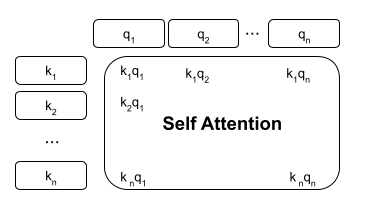
\includegraphics[scale=.6]{./images/selfAttention.png}
\caption[Jeff Yoshimi with consultation from Tim Meyer.]{Scaled self attention matrix generated from key and query vectors. Value vectors (not shown here) are then multiplied by this matrix to produce the output of one head of a block.}
\label{selfAttention}
\end{figure}

Within each block all the mechanisms above are separated out into multiple ``heads''. As a result, the network can learn \emph{multiple} ways to compare words in the sentence to each other, a bit like how a convolutional network (section \extref{convolutionalLayer}) develops \emph{multiple} filters to analyze an image. The results of these different attention heads are combined and as a result each layer of a transformer network involves a sophisticated representation of the sentence that represents multiple types of inter-word dependency. Number of heads per block corresponds to a more complex form of \glossary{representational width}.

% TODO: This part is not clear
This entire process happens once for each head. The outputs of all the heads are squashed back together and normalized, and put through a standard feed-forward network of the kind we've been talking about throughout the book. The output of the block is a set of vectors that has the same shape as the input vectors. See figure \ref{transformerArchitectureSchematic}.  For example, in the example in figure \ref{contextWindow} the input would be 9 vectors with 3 components each, and the output would be too. For a nice visualization that is vaguely in the Simbrain style, see \url{https://bbycroft.net/llm}.

\begin{figure}[h]
\centering
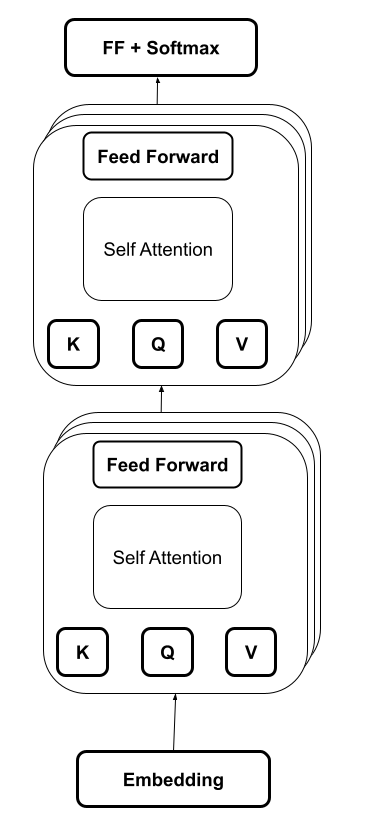
\includegraphics[scale=.45]{./images/transformerArchitectureSchematic.png}
\caption[Jeff Yoshimi with consultation from Tim Meyer.]{Schematic of the whole structure. Representational width (multiple heads) and depth (multiple stacked blocks) are both evident.}
\label{transformerArchitectureSchematic}
\end{figure}

Within each block all the mechanisms above are separated out into multiple ``heads''. As a result, the network can learn \emph{multiple} ways to compare words in the sentence to each other, a bit like how a convolutional network (section \extref{convolutionalLayer}) develops \emph{multiple} filters to analyze an image.  The results of these different attention heads are combined and as a result each layer of a transformer network involves a sophisticated representation of the sentence that represents multiple types of inter-word dependency.
 
 % Too much now?
Now we take a lesson from deep networks, and stack many of these transformer blocks on top of each other, to produce increasingly sophisticated representations.  This is \glossary{representational depth}. Recall that with deep networks for vision, we get features, features of features, features of these features, etc. whose activations match neural response properties of different layers of the human visual system. This builds on the old idea of the \emph{Pandemonium} model (section \extref{cog_rev}), which involved (at successive layers): edge detectors, detectors for combinations of edges, detectors for combinations of these combinations (e.g. fragments of letters), and ultimately letter detectors. In a similar way, the successive layers of a transformer model of language correspond to increasingly complex features of the input stream, including syntactic categories, semantic properties, and far more complex features as well.\footnote{The extent to which activation patterns correspond to syntactic or semantic features is measured using post-hoc interpretation techniques such as probing. As with so many other neural network features, these were not ``programmed in'' by the engineers, but are emergent from the network after training, and are studied and described by scientists after the fact.}  We return to this topic at the end of the chapter. The transformer model was not built to help cognitive science, after all, but to support NLP engineering tasks. Nonetheless, the results are so compelling that they are of interest to cognitive scientists.

The whole thing is trained using gradient descent and supervised learning (chapter \extref{ch_supervised}). It's the same ideas as with a simple feed-forward network, but with more things trained. Items in bold in the figures above are trained: the word embedding, the key, query, and value matrices for each head  in each block, and the normal weights and biases of the feed-forward networks.  Gradient descent is being pushed back through a \emph{lot} of stuff here!

\subsection{Softmax Outputs}

% Internal link to softmax once we have it; be sure temperature is discussed
The first step in a transformer is to embed inputs, as we've seen. The last step is to un-embed them. We do this with softmax outputs.

% Possibly merge in. Notice that since the target data are binary one-hot encoded labels, the task given this network can technically be seen as a classification task (section \extref{classificationRegression}). The network is classifying context window inputs into categories corresponding to what the next token should be. So, for any context window input, the output is a probability over next tokens, and one of the most probable next tokens is selected, and recursively added to the context window as described above. However, even though training involves a classification task, in practice these models are not thought of as classifiers, since they are not used in that way; they are not used to ``classify'' inputs the way something like an image classifier is (like a model that distinguishes cats and dogs in pictures), but rather to generate text sequences (also, there is a lot more machinery involved in a standard LLM, like models that determine when a response should be terminated). Thus these are not thought of as classifiers in practice, even though at their heart they include a classification task.

In figure \ref{nextWordPrediction} to make it clear that we were predicting the next word we just showed the same word embedding in the input and output.  However, it turns out that in practice, one-hot encodings are usually used over the whole vocabulary, so that the actual training is a classification task. However, classification is here a kind of \emph{proxy task}. Our actual task is predict a set of probabilities over next tokens.  The interesting thing is that by \emph{trying} to perfectly classify next tokens (an impossibly task), we end up with good probabilities, which is exactly we're after.\footnote{Here is a way to think of it. If the model was trained to 100\% accuracy on the classification task, then it would always generate the same sentences from the same prompts (because it would assign one unique token to the current input). But then it could not generate new instances of text.}

 Thus the output of an LLM will often by a layer with around 50,000 outputs in a \glossary{softmax} layer, where the output indicates how probable a token in a given language is, as the next token, given the input (all the prompts and responses in the context window so far are). See figure \ref{contextWindow} for how this might look for our simple example, where the output vocabulary just contains 7 tokens.

\begin{figure}[h]
\centering
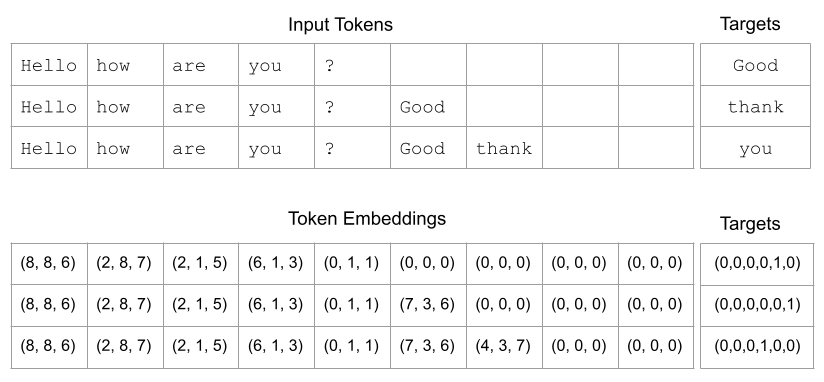
\includegraphics[scale=.45]{./images/contextWindow.png}
\caption[Jeff Yoshimi]{What some training data might look like for the example in figure \ref{gptRecursedInputs}. The top row panel shows the tokens in three training examples and the bottom row shows the corresponding token embeddings.  It should be clear that the bottom panel shows inputs that can actually be fed into a neural network, in this case, a network with 27 input nodes. Note that the targets are one-hot encoded, because these networks are actually classifiers. They have one ``node'' for each token in this small vocabulary. In this case, there are 7 nodes for the 7 tokens: ``Hello'', ``how'', ``are'', ''you'', ``?'', "Good'', ``thank''.  }
\label{contextWindow}
\end{figure}

% This can be controlled using the softmax temperature parameter, where higher temperatures make the outputs more random or ``creative''
Once we have a probability distribution over tokens, we select one of the most probable next tokens and that becomes the output. This is usually done by sampling from among the top $n$ most probable next tokens. Thus the final softmax layer does the opposite of what the embedding layer does. Rather than converting from tokens to activations, it converts from activations to tokens, and is thus a ``de-embedding'' layer.

\subsection{Other tricks and features}

There are also a number of other tricks in the whole process.\footnote{In particular positional encodings, a special form of vector that can be added to a word embedding that tags it for its location in a sequence. Since words are intrinsically tagged with their position, they can be processed in parallel, which allows the architecture to run on fast parallel hardware. A kind of feature engineering trick (chapter \extref{ch_data_science}).  }

As with any supervised learning algorithm, there are \glossary{hyperparameters} to take care of. Some of the hyperparameters for GPT-3 are shown in figure \ref{gptParams}. Some are familiar, like learning rate. Others describe number of layers. Others the number of heads. All are large and much larger with GPT-4.

%TODO: Check all this.  Would be good to make sure each hyperparameter is explained and referenced somewhere. t $d_model$ is the embedding dimension .

\begin{figure}[h]
\centering
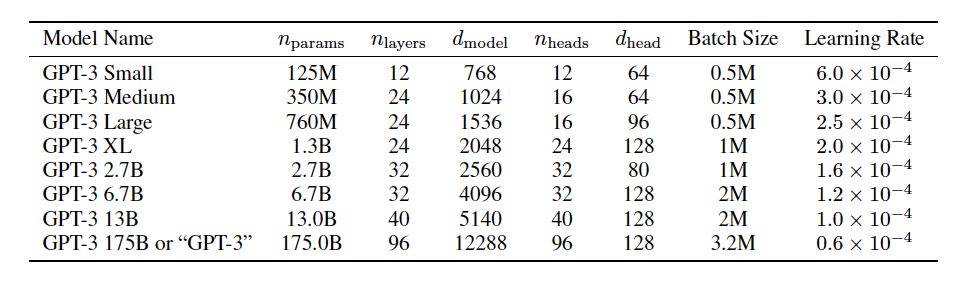
\includegraphics[scale=.4]{./images/gpt3_params.png}
\caption[GPT Technical report. Todo]{Some of the hyper-parameters used in training different versions of GPT-3. Some of these are familiar to us, others are new. Notice the number of parameters, which are primarily weights and biases.  Billions, and GPT-4 is approaching 2 trillion parameters.  That is a lot of weights and biases.  Our xor 2-2-1 network had 3 biases and 6 weights, 9 parameters.  A standard convolutional neural network might have millions of parameters. So this is just massively larger. }
\label{gptParams}
\end{figure}

%TODO: Where? One shot, zero shot etc. Lots of the "shot" learning is based on reasoning  (through the width and depth of the giant network), getting it to reason step by step through something. It is not weights and biases.  Background of one shot in AI vs. NN. NN require gradual learning but humans learn in one shot so that was a problem. And classical AI can do so too just with a single rule in the database

%\section{Interpretation and Evaluation}
%
%There is something strange about LLMs.  They were built by humans but are so complex that we do not completely understand them. This has often been the case historically with neural networks, but the issue is accentuated here. It's like we built this super powerful motor and now we can put it in different things, but we don't understand how the motor works so we have to look at its components and find new ways to study it, reverse engineer it, use it, etc. This may be a difference of degree (CNNs were also like this), but it is enough of a difference in degree that it feels like a change in kind.\footnote{One aspect of this is that with CNN's one could run a bunch on their own computer; with LLMs they are so expensive to train and it takes so long that people just make API calls to existing LLM models. So it feels more like this separately existing thing is just being studied, akin to studying any natural phenomenon in nature.} It really does feel different. These massive transformer-based neural networks with all their many layers and blocks and matrices and other features somehow magically produce human-like speech and video, etc., but how exactly is not understood. 
%
%The point was made striking early via BERT (which came out around the time of GPT-2). It came out of Google and fit their engineering needs. Psychologists and linguists then realized  BERT was doing better at analyzing language than other models in linguistics, so they started to treat it as an object of scientific interest in its own right. This gave rise to a new field called ``BERTology''. 
%
%As a result of this feature of LLMs, a huge ecosystem of analysis is growing up around them. Not all of it is obviously relevant to our focus here, cognitive science, but much of it is potentially relevant and it's too early to tell, so we here give a brief review.
%
%Topics  include prompt engineering, pre-training, adaptation tuning, utilization, and capacity evaluation.
%
% Fine tuning. Fine tuning is updating an already existing LLM to bias it in favor of the language in some specified corpus you are interested in. For example you might download a llama 2 model, and then fine tune it based on a set of corpus using x library.  See Kauf and Ivanova 2023
% Video on fine tuning an LLM to talk about a set of PDFS (we can do it on Husserl): https://www.youtube.com/watch?v=dXxQ0LR-3Hg
%
% In context learning are things you can add to your prompt, ie in the context window, to improve the output, will be discussed further in the prompt engineering chapter
% 
% Use of external functionalities like wolfram alpha
%
% Prompt engineering. Prompt templates. Prompting techniques. Funny historical examples of prompting discoveries
%
%https://developer.nvidia.com/blog/how-to-get-better-outputs-from-your-large-language-model/
%
%https://arxiv.org/pdf/2310.14735.pdf


% NOT SURE WHERE BERTOLOGY STUFF
%
%
%In a paper titled ``A Primer in BERTology: What We Know About How BERT Works'' \cite{rogers2020primer}, a ``survey of over 150 studies of the popular BERT model'',  the authors explain:
%\begin{quote}
%Although it is clear that BERT works remarkably well, it is less clear why, which limits further hypothesis-driven improvement of the architecture. Unlike CNNs, the Transformers have little cognitive motivation, and the size of these models limits our ability to experiment with pre-training and perform ablation studies. This explains a large number of studies over the past year that attempted to understand the reasons behind BERT’s performance. In this paper, we provide an overview of what has been learned to date, highlighting the questions that are still unresolved.
%\end{quote}
%This is a strange situation. Engineers built something and then scientists created a science to understand it!  
%
%Even before GPT-3 hit the world, transformer-based LLMs were making a huge impact in the world of computational linguistics, via BERT, already mentioned. 
%
%In a paper co-authored by Jay McClelland  \cite{mcclelland2020placing} (a member of the original PDP group at UCSD; see section \extref{first_resurgence}), the following example is used to illustrate the point:
%\begin{quote}
%John put some beer in a cooler and went out with his friends to play volleyball. Soon after he left, someone took the beer out of the cooler. John and his friends were thirsty after the game, and went back to his place for some beers. When John opened the cooler, he discovered that the beer was \rule{1cm}{0.15mm}.
%\end{quote}
%The reader expects the word ``gone'' next, but if ``took the beer'' is replaced with ``took the ice'' the reader expects something like ``warm''. But the first part of the sentence is too far apart from the last part for an unrolled backprop through time network to pick up the relationship.  Transformer networks like BERT overcome this problem.
%
%The big questions are: how exactly does BERT do this, and whatever it does, is it relevant to human language processing?  This creates a fascinating twist on our earlier discussion of types of neural network research (section \extref{typesOfResearch}). Recall that neural networks are sometimes used for engineering, sometimes for science, but that there is a feedback between these categories of research. For example, deep convolutional networks originated in scientific studies of visual processing, got refined and used for pattern recognition tasks in engineering, and the resulting deep networks were so powerful that they were then taken back into science  to describe (for example) the human visual system.

% TODO: Rename label
\section{Relevance to cognitive sciences}\label{sect_bert}
% Saliency maps (polyphony's talk)

At this point transformer-based LLMs are a major object of study in many academic disciplines and areas of cognitive science. Here are some representative examples.

\subsection{LLMs and Linguistics}

The training task for BERT differs from other contemporary language models; BERT uses ``masked language modeling'' (MLM) instead of traditional next-word prediction.\footnote{See \cite{devlin2018bert} for a detailed explanation.} Instead of modeling language as a left-to-right stream of words, where the model predicts the next-word based on the previous context, BERT instead masks a token in the middle of the sentence, and predicts it based on the surrounding sentential context. This is advantageous over unidirectional left-to-right and concatenated left-to-right and right-to-left models, since it creates a truly bidirectional representation where the left and right contexts are joined together.

Research has also considered how these models handle syntax and semantics, revealing insights that bridge computational models and linguistic theory. One key study (``What Does BERT Look At? An Analysis of BERT's Attention'') investigates the attention patterns in BERT and their correspondence to linguistic phenomena. This study found that BERT's attention heads often focus on specific linguistic roles, such as the direct objects of verbs or the determiners of nouns. Interestingly, some attention heads display broad attention across entire sentences, while others are highly focused, suggesting a complex, multi-faceted approach to language understanding within the model. 

\subsection{LLMs and Neuroscience}

Just like Yamins and DiCarlo used convolutional neural networks (CNNs) to predict brain activity (section \extref{cnn_applications}), researchers are now leveraging transformer-LLMs to understand how our brains process language. 

Schrimpf and colleagues \cite{schrimpf2021neural} explore how LLMs, like GPT and BERT, can predict neural responses during language comprehension. They proceeded by comparing  brain activity of participants reading or listening to sentences with the activity patterns generated by these modelsOne of their key findings is that transformer models, especially GPT, can predict nearly 100\% of the explainable variance in neural responses to sentences! 

An interesting aspect of this study is the comparison between GPT and BERT. GPT, which processes language in a unidirectional manner (predicting the next word based on the previous words), was found to outperform BERT, which uses a bidirectional approach (considering the context from both directions). So it looks like our brain rather predicts unidirectionally! This makes sense given that we usually are confronted with language orally and so get ``fed'' sentences word by word. This result accordingly provides evidence for a theory of neuroscience called \emph{predictive processing}, which suggests that the brain is constantly making predictions about incoming sensory information to facilitate comprehension.

\subsection{LLMs and philosophy}

%A lot of research exists on better understanding how LLM works internally (see BERTology as a primer; now Anthropic AI do great work). Another important line of research is to better assess their capabilities (see BIG-bench paper). Here, behavioral sciences have played a very interesting role. Indeed, behavioral sciences have developed rigorous ways to test cognitive abilities, such as intelligence, given only the behavior of an agent. This comes in handy to benchmark LLMs!
%
%See Using cognitive psychology to understand GPT-3 by Marcel Binz and Eric Schulz.

% TODO: Stochastic parrot original
Philosophers are also interested in LLMs for the obvious reason that they have completely changed the game and even passed the Turing Test. A subject that generates a lot of debate is the capacity of these models to ``understand language''. Here the discussion is still very much shaped by philosophical arguments that a machine can’t get the ``meaning'' of a word just by manipulating meaningless symbols. After an article by Emily Bender and colleagues \cite{bender2021dangers}, it has become common to say that LLMs are mere ``stochastic parrots'' that capture nothing more than mere co-occurrence probabilities. Many philosophers agree with this view. However, others argue that LLMs do get the meaning of words (but we won’t get into any details here). In any case, the impressive results of models such as chatGPT fundamentally question not only empirical insights about language but also very deep philosophical conceptions about language.

% TODO: Octopus test